\documentclass[10pt, a4paper,twocolumn]{article}
\usepackage[latin1]{inputenc}
\usepackage{amsmath}
\usepackage{amsfonts}
\usepackage{amssymb}
\usepackage{graphicx}
\usepackage{xcolor}



\title{Toxic Comment Classification - Report}

\author{Mick van Hulst \and Dennis Verheijen \and Roel van der burg \and Brian Westerweel \and Joost Besseling}

\begin{document}
	\maketitle
	
	
	\section{Problem statement}
	We have chosen the toxic comment classification challenge on Kaggle. For this challenge we have to classify about 160000 comment. There are 6 different classes and each comment can be labeled with any of these classes. This means our problem is a multilabel classification problem.
	
	\section{Dataset}
	
	The dataset that is provided by Kaggle consists of some 160000 comments with their respective class labels. They also provide a test set of about the same size, without the labels. Our task is to predict the labels of the test set.
	%TODO een voorbeeld sample
	
	One important characteristic of our data is that the set is very imbalanced. This posed many challenges to us.
	
	\begin{figure}[h]
		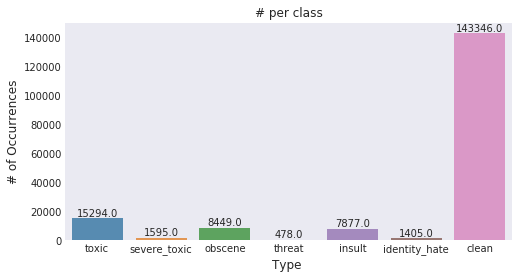
\includegraphics[width=0.4\textwidth]{img/distribution_histogram}
		\caption{Figure from Kaggle \cite{abc}}
	\end{figure}
	%TODO name the challenges
	
	
	\subsection*{Data Preprocessing}
	
	Since the data consists of raw Wikipedia comments, we have to do some preprocessing to convert the words to lowercase and change words that are spelled erroneously to the correct spelling. We use the TweetTokenizer to handle this for us.
	
	\section{Feature based models}
	\subsection{Feature Extraction}
	Our first approach was to look at the data and try to extract some features by hand. These features include things like: 
	\begin{itemize}
		\setlength\itemsep{0px}
		\item Ratio of capitals vs total characters
		\item Ratio of punctuation characters
		\item Total length in characters, words and in sentences
		\item Total amount of some special characters: ?, (, ), ! and some other characters.
		\item Amount of unique words		
	\end{itemize}
	In total we produced about ten features.
	
	We used these features to train various other models on. We will evaluate each model seperately, but in the end, none of these feature based models managed to produce convincing results.
		\subsection{Models}
	\subsection{Feature Extraction Part 2}
	
	After a meeting with our supervisor, we thought that a problem with our feature extraction was that we might be using to little features. Since we are trying to predict 6 classes seperately, and we are using a quite complex set, the dimensionality of the set is probably higher than 10. That is why we decided to introduce some extra features.
	
	\begin{itemize}
		\item For a list of swear words (since we are doing \emph{toxic} comment classification), we added a feature denoting whether that particular word occurred in the comment.
		\item {\color{red}More features??} 
	\end{itemize}
	
	
	\section{Neural Networks}
	
	Having implemented these feature based approaches, we decided it might be better to use a neural network model. We decided to use the LSTM (Long Short Term Memory), because LSTM's are recurrent neural networks, so it can learn the context of words in sentences. First we tried to use the most simple LSTM we could think of.
	
	%TODO describe this lstm and its aoc
	
	After that, we found  very well performing LSTM based approach on Kaggle (a bidirectional LSTM). This means that we feed the sentence twice to the LSTM, once normally, from front to back, and once flipped.
	\begin{figure}
	\begin{verbatim}	
	    A forward and backwardsentence
	    sentence backward and forward A
	\end{verbatim}
	\caption{An example of how the  Bidirectional layer would feed the data to the LSTM}
	\end{figure}
	
	
	We implemented a 1 dimensional convolutional neural network.
	
	

	
	\section{Validation}
	
	
	\section{Next Steps}
	After the first competition, we have already learned many things. 
	
	\subsection{Data handling}
	
	\subsection{Ensemble}
	
	\subsection{Division of tasks}
	
	
	\begin{thebibliography}{xx}
		\bibitem{abc}
		\textsc{Jagan}, \textit{Stop the S@\#\$ - Toxic Comments EDA},
		 https://www.kaggle.com/jagangupta/stop-the-s-toxic-comments-eda
		
			
		
	\end{thebibliography}
	
\end{document}